\documentclass{beamer}
\usepackage{biblatex}
\usepackage{amsmath}
\usepackage{braket}
\usepackage{amssymb}
\usepackage{siunitx}

%Graphics and Videos
\usepackage{graphicx} %The mode "LaTeX => PDF" allows the following formats: .jpg  .png  .pdf  .mps
\graphicspath{{./images/}} %Where the figures folder is located
\usepackage{media9}
\addmediapath{./videos/}

\addbibresource{refs.bib}

\usetheme{Boadilla}
\title{Cavity QED mit Mikrowellen Resonanz}
\subtitle{Nobel Preis (2012) von Serge Haroche}
\author{Angelo Brade}
%\institute{Rhenish Friedrich Wilhelm University of Bonn}
\institute{University of Bonn}
\date{\today}


\makeatother
\setbeamertemplate{footline}
{
  \leavevmode%
  \hbox{%
  \begin{beamercolorbox}[wd=.2\paperwidth,ht=2.25ex,dp=1ex,center]{author in head/foot}%
    \usebeamerfont{author in head/foot}\insertshortauthor
  \end{beamercolorbox}%
  \begin{beamercolorbox}[wd=.4\paperwidth,ht=2.25ex,dp=1ex,center]{section in head/foot}%
    \usebeamerfont{section in head/foot}\insertsectionhead
  \end{beamercolorbox}%
  \begin{beamercolorbox}[wd=.4\paperwidth,ht=2.25ex,dp=1ex,center]{title in head/foot}%
    \usebeamerfont{title in head/foot}\insertshorttitle\hspace*{1em}
    \insertframenumber{} / \inserttotalframenumber\hspace*{1ex}
  \end{beamercolorbox}}%
  \vskip0pt%
}
\makeatletter
\setbeamertemplate{navigation symbols}{}



\begin{document}
\begin{frame}
	\titlepage
\end{frame}
\begin{frame}
	\frametitle{Outline}
	\tableofcontents
\end{frame}

\section{Historische Einordnung}
\subsection{Vorrangegangene Entwicklungen}
\begin{frame}{Vorrangegangene Entwicklung}
	\begin{itemize}
		\item Einstein, Schrödinger, etc. hatten nur Gedankenexperimente von einzelnen QM Zuständen (1930)
		      \begin{itemize}
			      \item reales Experiment undenkbar
			      \item nur Theorie
		      \end{itemize}
		\item bisher nur Experimente mit den "Überresten" möglich (Ionisationsspuren, etc.)
		      \begin{itemize}
			      \item \textbf{Teilchen/Zustand} wurde dabei \textbf{zerstört}
		      \end{itemize}
	\end{itemize}
\end{frame}
\subsection{Schrödingers Katze}
\begin{frame}
	\frametitle{Schrödingers Katze}
	\begin{columns}
		\begin{column}{0.5\textwidth}
			\begin{itemize}
				\item Tod von Zustand des Teilchens abhängig
				\item Teilchen in Superposition
				\item $\Rightarrow$ Katze mit Teilchen verschränkt
				\item Box wird geöffnet $\Rightarrow$ Zustand kollabiert
			\end{itemize}
		\end{column}
		\begin{column}{0.5\textwidth}
			\begin{figure}
				\center\includegraphics[width=1\textwidth]{images/scat.png}
				\caption{Schrödingers Katze\cite{lect}}
			\end{figure}
		\end{column}
	\end{columns}
\end{frame}
\subsection{Prinzip}
\begin{frame}{Prinzip}
	\begin{columns}
		\begin{column}{0.5\textwidth}
			\begin{itemize}
				\item Serge Haroche (geb. 1944)
				\item Ziel: Beobachtung von einzelnden Teilchen, ohne sie zu zerstören
				\item
				\item Nutzt Jaynes-Cummings Modell und QND
			\end{itemize}
		\end{column}
		\begin{column}{0.5\textwidth}
			\begin{figure}
				\center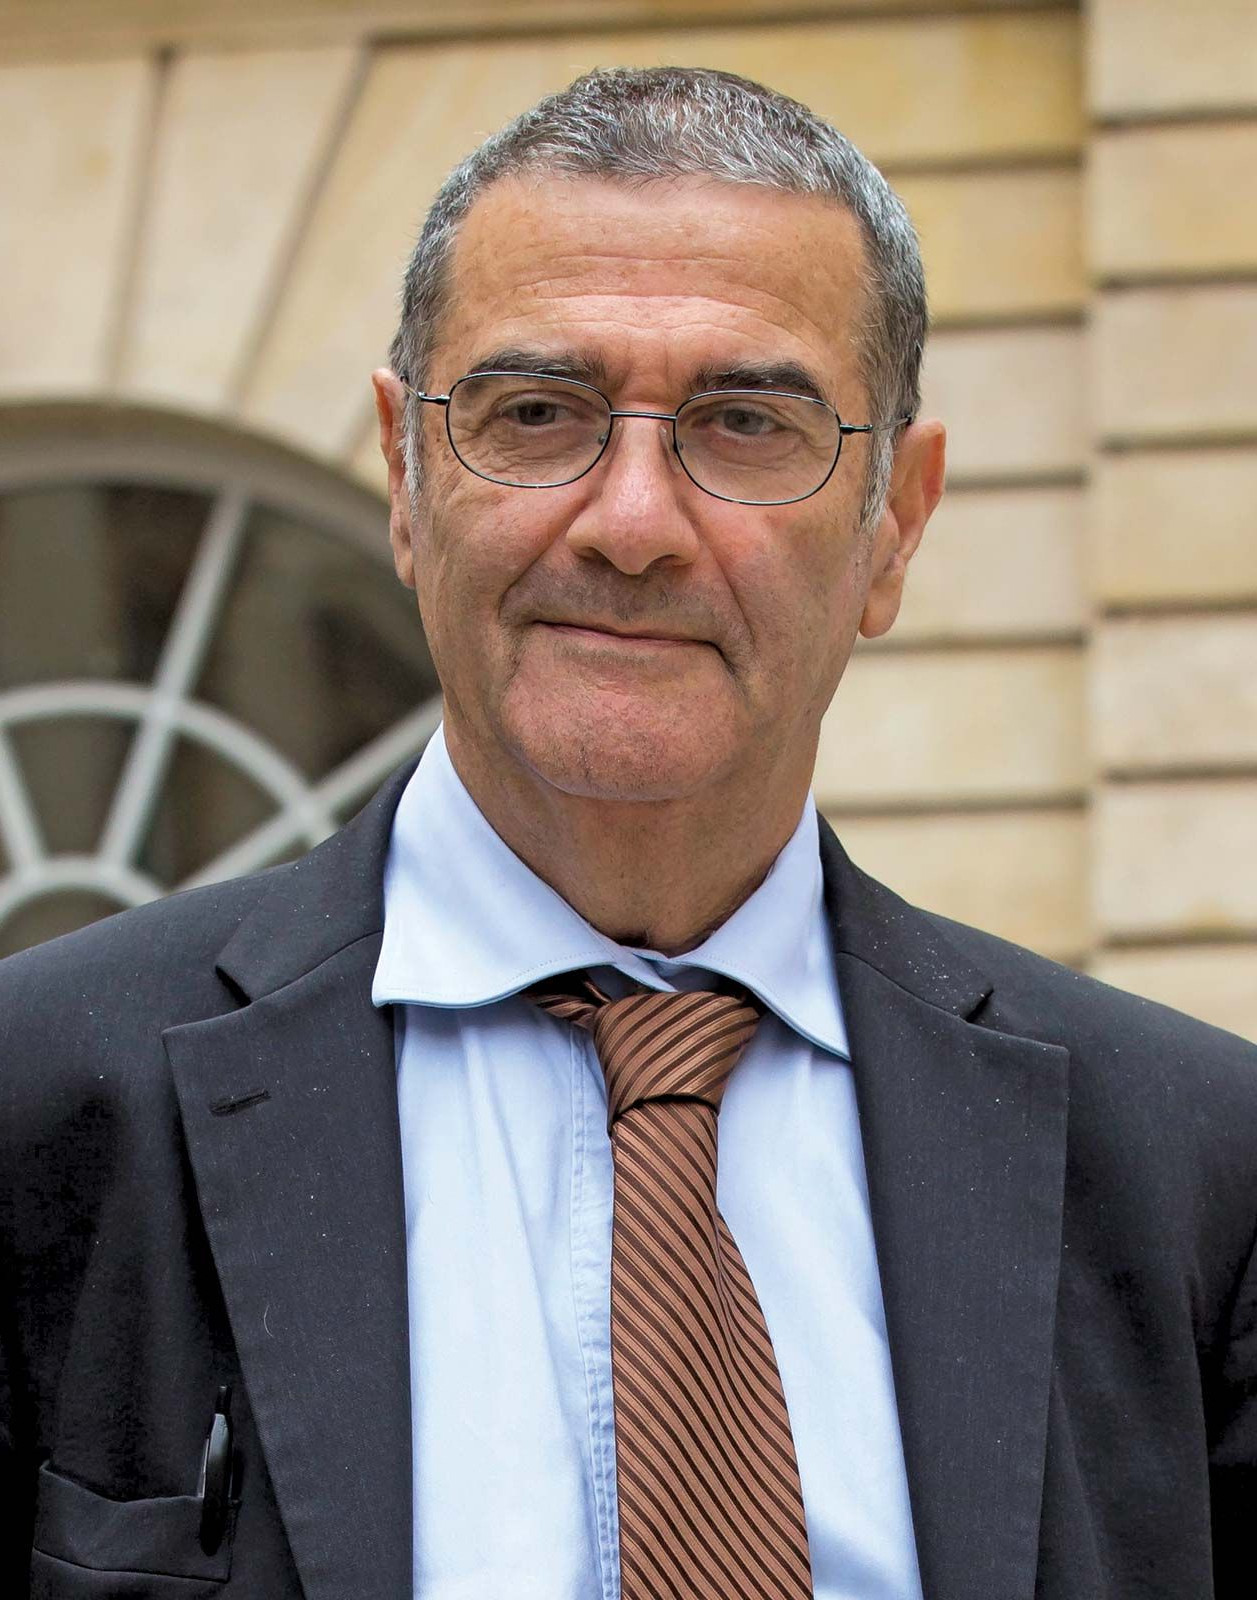
\includegraphics[width=.8\textwidth]{images/haroche.jpg}
				\caption{Serge Haroche\cite{brit}}
			\end{figure}
		\end{column}
	\end{columns}
\end{frame}
\begin{frame}{Jaynes-Cummings Modell}
\end{frame}
\begin{frame}{Prinzip}
	\begin{figure}
		\center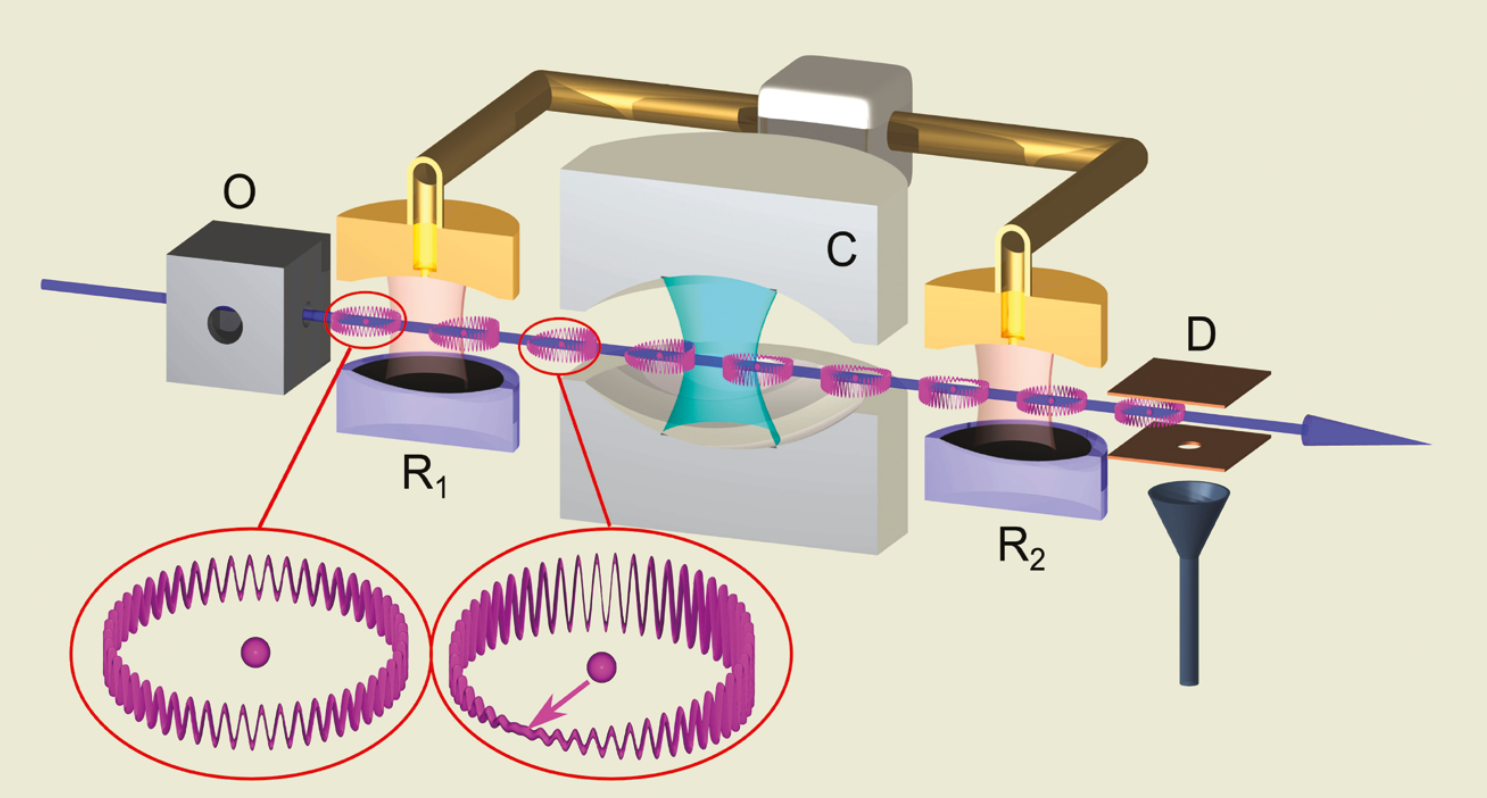
\includegraphics[width=1\textwidth]{images/aufbau.png}
		\caption{cQED Aufbau mit Ramsey Interferometer\cite{lect}}
	\end{figure}
\end{frame}
\section{Mikrowellen Resonator}
\subsection{Stehende Wellen und Moden}
\begin{frame}{Stehende Wellen}
	\begin{enumerate}
		\item Einlaufende Welle
		      \begin{itemize}
			      \item $E_1=A e^{i(\omega t - kx)}$
		      \end{itemize}
		\item Reflexion
		      \begin{itemize}
			      \item Umkerhung der Phase $kx \rightarrow -kx$ und Phasenverschiebung $\pi$
		      \end{itemize}
		\item Auslaufende Welle
		      \begin{itemize}
			      \item $E_1 \rightarrow E_2=A e^{i(\omega t + kx + \pi)}$
		      \end{itemize}
		\item Interferenz nach Superpositionsprinzip
		      \begin{itemize}
			      \item $E_{\text{tot}} = E_1 + E_2 = 2Ae^{i(\omega t+\frac{\pi}{2})}\cos{(kx+\frac{\pi}{2})}$
			      \item $\Rightarrow y(x,t)=\text{Re}(E_{\text{tot}})=2A\sin{(\omega t)}\sin{(kx)}$
		      \end{itemize}
	\end{enumerate}
	\begin{figure}
		\center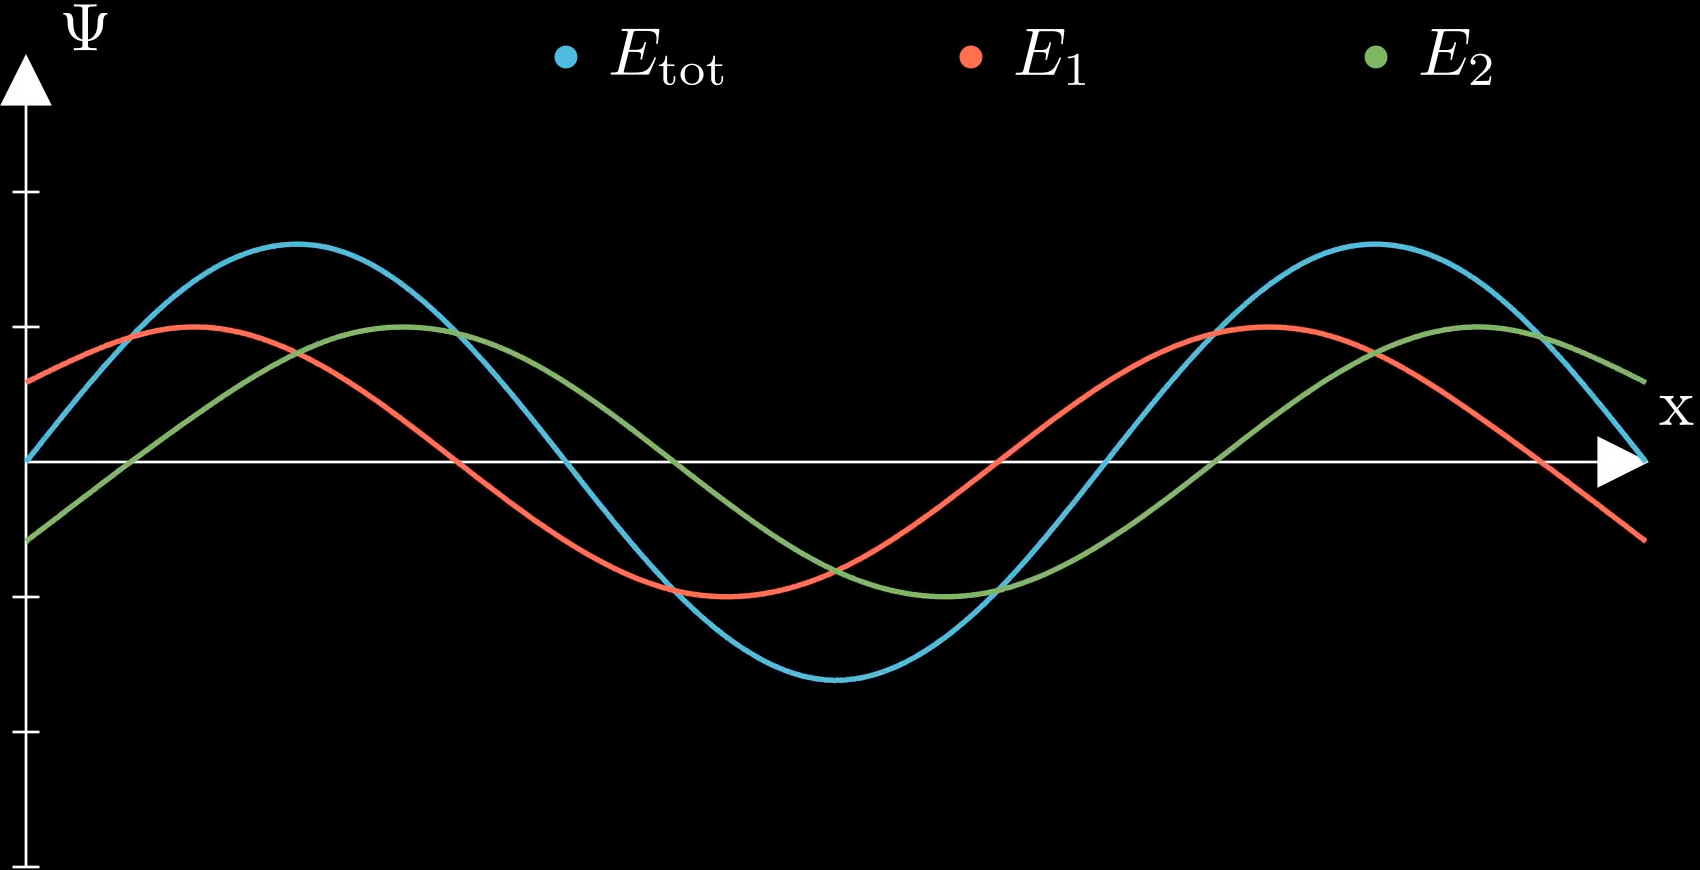
\includegraphics[width=0.5\textwidth]{images/schwebung.png}
	\end{figure}
\end{frame}
\begin{frame}{Moden}
	\begin{itemize}
		\item Mode: $y(x,t)=\text{Re}(E_{\text{tot}})=2A\sin{(\omega t)}\sin{(kx)}$
		      \begin{itemize}
			      \item mit $k=\pi\cdot m$, $m\in \mathbb{N}$
			      \item für $v_{\text{gr.}}=c=1 \Rightarrow k=\omega$
		      \end{itemize}
	\end{itemize}
	\begin{figure}
		\center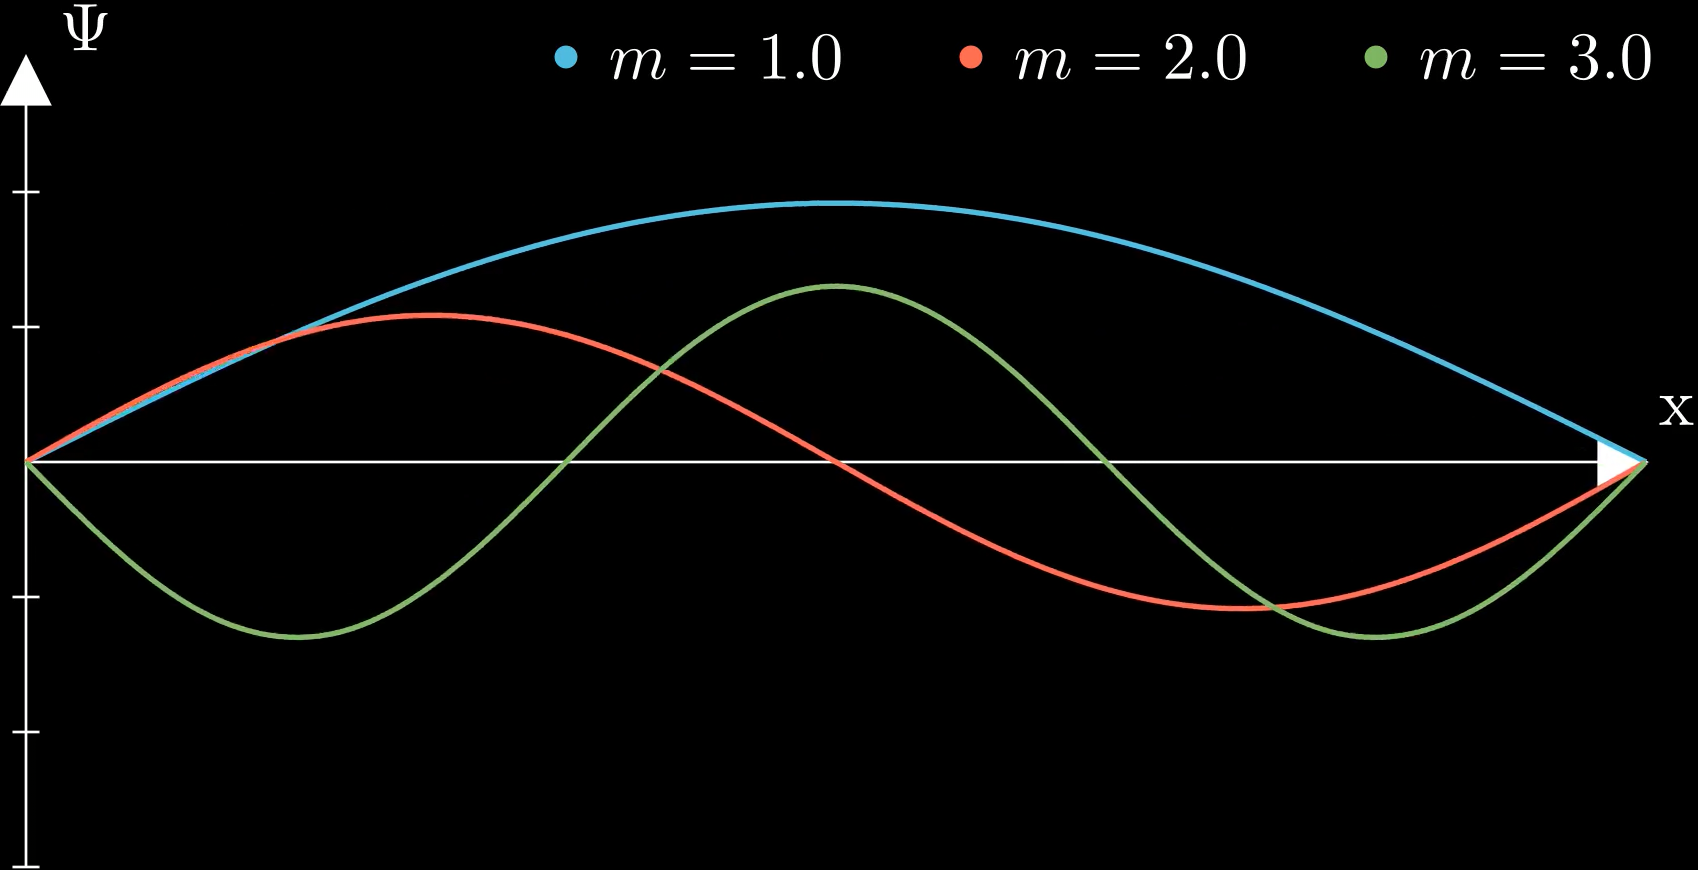
\includegraphics[width=0.8\textwidth]{images/harmonics.png}
	\end{figure}
\end{frame}
\subsection{Spiegel}
\begin{frame}{Spiegel}
	\begin{figure}
		\center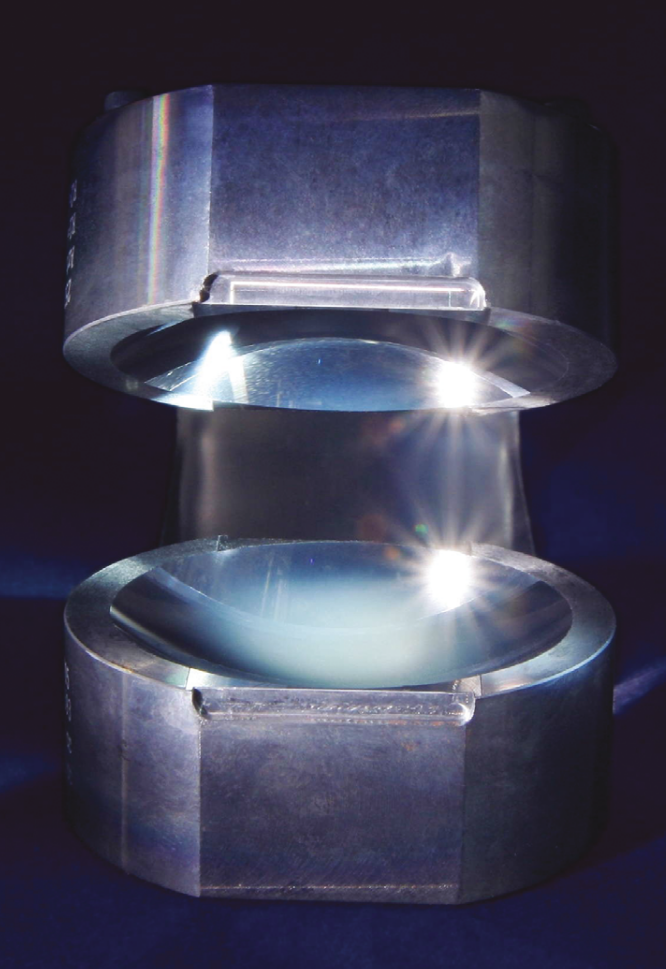
\includegraphics[width=.4\textwidth]{images/pbox.png}
		\caption{Photonbox\cite{lect}}
	\end{figure}
\end{frame}
\begin{frame}{Spiegel}
	\begin{itemize}
		\item Luft und Spiegel können als Leiter betrachtet werden
		\item Reflektionskoeffizient: $r=\frac{Z_A-Z_W}{Z_A+Z_W}$
		      \begin{itemize}
			      \item $Z_A$:=Abschlusswiderstand
			      \item $Z_W$:=Wellenwiderstand
		      \end{itemize}
		\item Für Metalle gilt: $Z_M=\sqrt{\frac{i\omega\mu}{\sigma+i\omega\epsilon}}$ mit $\sigma$:=Leitfähigkeit
		\item Spiegel (Abschluss) aus Metall: $Z_A=Z_M$
		\item $\Rightarrow \lim_{\sigma\rightarrow\infty}r=-1$
	\end{itemize}
\end{frame}
\subsection{Q Faktor}
\begin{frame}{Q Faktor: Güte}
	\begin{itemize}
		\item $Q:=\frac{\text{gespeicherte Energie}}{\text{Energieverlust}}$
		\item $r\rightarrow \pm1\Leftrightarrow Q\rightarrow\infty$
		\item Spiegel von Haroche: $Q \approx 10^6 \hat{=} \tau_{\gamma}\propto 10^{-3}$s
		      \begin{itemize}
			      \item \textbf{Zu niedrig}
		      \end{itemize}
		\item Bandbreite $B\propto\frac{1}{Q}$
		      \begin{itemize}
			      \item geringere Bandbreite $\Rightarrow$ Mode trifft Resonanzfrequenz besser
		      \end{itemize}
		\item $\Rightarrow$ \textbf{Leitfahigkeit soll maximiert werden}

	\end{itemize}
\end{frame}
\begin{frame}
	\Large\center Wie kann man die Leitfähigkeit erhöhen?
\end{frame}
\begin{frame}{Q Faktor: Meschede}
	\begin{columns}
		\begin{column}{0.5\textwidth}

			\begin{itemize}
				\item Spiegel von Meschede: $Q \approx 10^{10} \hat{=} \tau_{\gamma}\propto10^1$s
				      \begin{itemize}
					      \item nutzt \textbf{Supraleiter} $\Leftrightarrow Z_M \approx 0 \Leftrightarrow r\approx-1$\
				      \end{itemize}
				\item Haroche nutzt Spiegel von Meschede
				\item Meschede wird Postdoc von Haroche
			\end{itemize}
		\end{column}
		\begin{column}{0.5\textwidth}
			\begin{figure}
				\center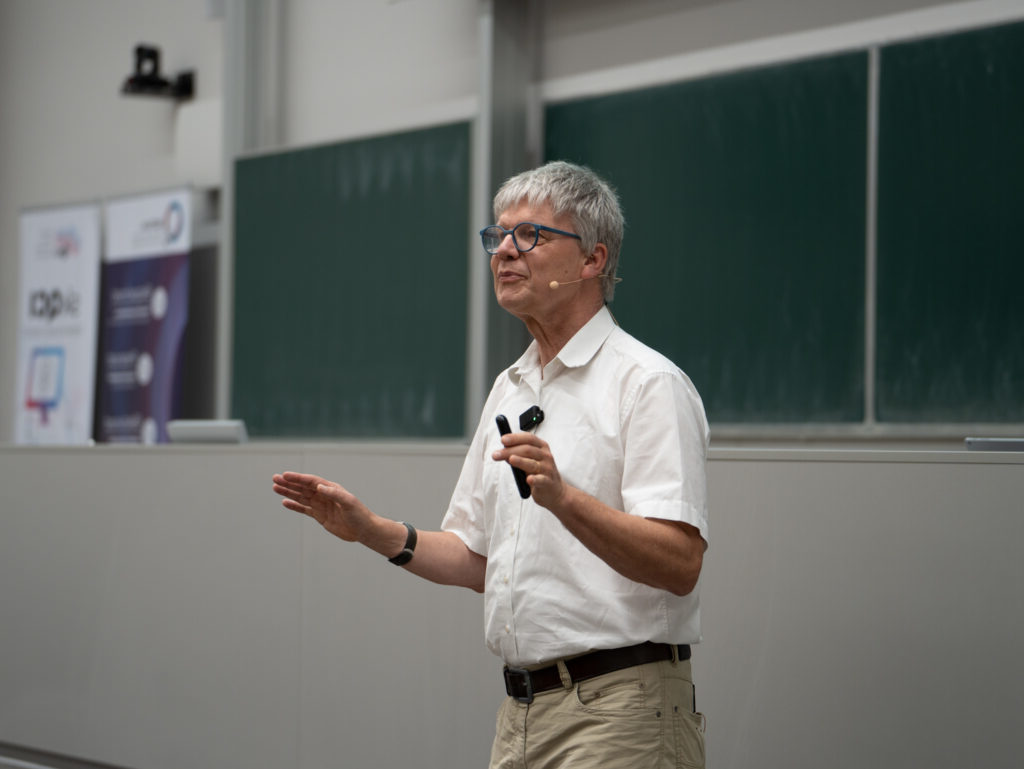
\includegraphics[width=1\textwidth]{images/meschede.png}
				\caption{Dieter Meschede\cite{qute}}
			\end{figure}
		\end{column}
	\end{columns}
\end{frame}
\section{QND}
\begin{frame}{Quantum nondemolition (QND) measurement}
	\begin{figure}
		\center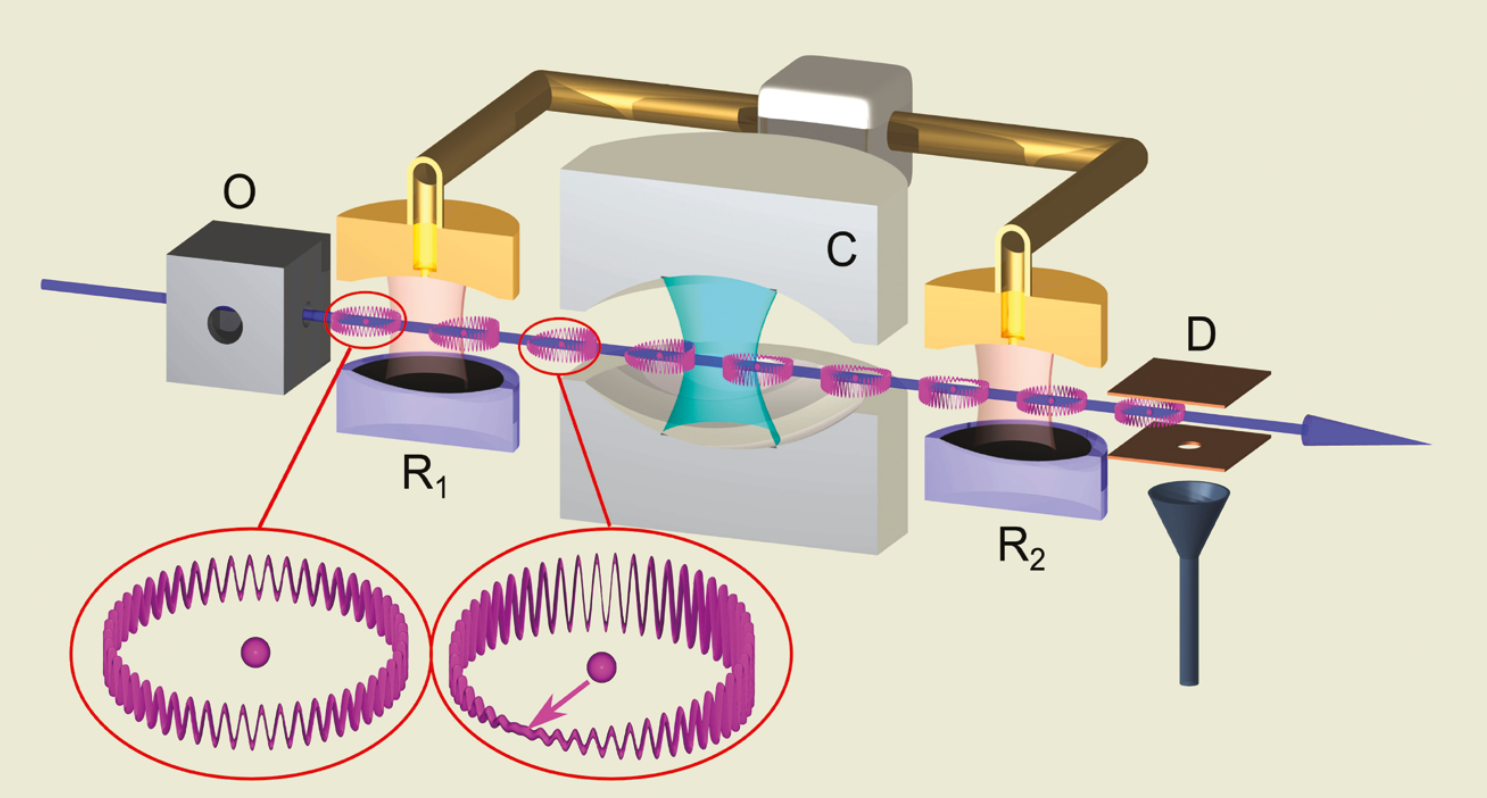
\includegraphics[width=1\textwidth]{images/aufbau.png}
		\caption{cQED Aufbau mit Ramsey Interferometer\cite{lect}}
	\end{figure}
\end{frame}
\subsection{Rydberg-Atom}
\begin{frame}{Rydberg-Atom}
	\begin{columns}
		\begin{column}{0.5\textwidth}
			\begin{itemize}
				\item Atom: stark angeregte $e^-$
				\item hier: $e^-$ in $n=50$ und $n=51$ Orbital
				      \begin{itemize}
					      \item $\ket{g}=\ket{n=50}$ und $\ket{e}=\ket{n=51}$
					      \item schnelle Oszillation\\$\Rightarrow\approx$ monopol (uniforme Welle)
				      \end{itemize}
				\item $\frac{1}{\sqrt{2}}(\ket{g}+\ket{e})\Rightarrow$ Schwebung
				      \begin{itemize}
					      \item Störung ist analog zu Spin Resonanz mit $\pi/2$-RF Puls
					      \item Schwebung: $f=\SI{51}{GHz}\Rightarrow$ dipol
				      \end{itemize}
				\item Photon präsent $\ket{g}$ und $\ket{e}$ werden leicht verschoben $\Rightarrow f\neq\SI{51}{GHz}$
			\end{itemize}
		\end{column}
		\begin{column}{0.5\textwidth}
			\begin{figure}
				\center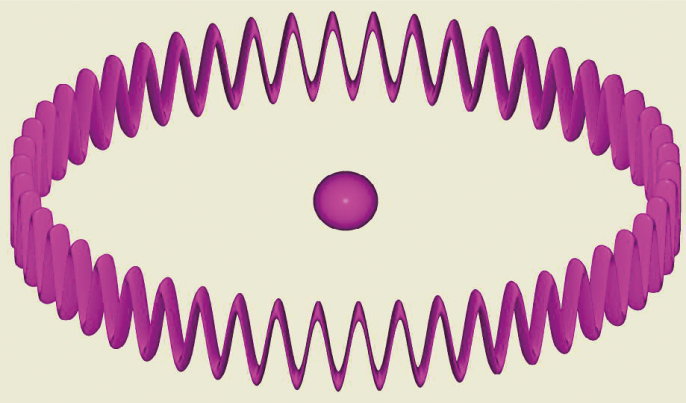
\includegraphics[width=.75\textwidth]{images/uniwave.png}
				\caption{Uniforme Welle\cite{lect}.}
			\end{figure}
			\begin{figure}
				\center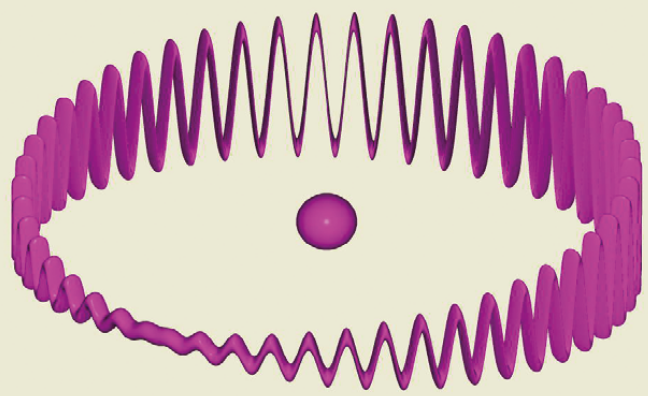
\includegraphics[width=.75\textwidth]{images/dipwave.png}
				\caption{Dipol Welle\cite{lect}.}
			\end{figure}
		\end{column}
	\end{columns}
\end{frame}
\begin{frame}{RF-Puls}
	\begin{columns}
		\begin{column}{0.5\textwidth}
			\begin{enumerate}
				\item zwei niveau System $\Leftrightarrow$ Bloch-Kugel
				\item $\pi/2$-Puls "klappt" $\ket{g}\rightarrow\frac{1}{\sqrt{2}}(\ket{g}+\ket{e})$ um
				\item Phase $\phi$ präzidiert
				      \begin{itemize}
					      \item Photon präsent: $\phi\rightarrow2\pi$
					      \item Photon abwesend: $\phi\rightarrow\pi$
				      \end{itemize}
				\item R2 Puls "klappt" mit $\pi/2$-Puls nach
				      \begin{itemize}
					      \item nach oben ($\phi=2\pi$)
					      \item nach unten ($\phi=\pi$)
				      \end{itemize}
			\end{enumerate}
		\end{column}
		\begin{column}{0.5\textwidth}
			\begin{figure}
				\center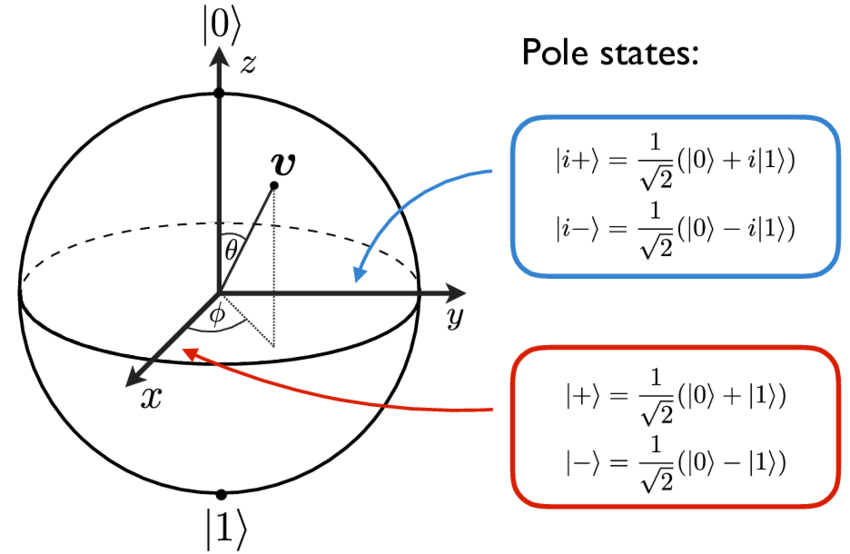
\includegraphics[width=1\textwidth]{images/blochkugel.png}
				\caption{Blochkugel\cite{qi}.}
			\end{figure}
		\end{column}
	\end{columns}
\end{frame}
\subsection{Ramsey Interferometer}
\begin{frame}
	\frametitle{Ramsey Interferometer}
	\begin{enumerate}
		\item R1: $\pi/2$-Puls für Superposition
		\item Cavity: ändert Präzidierung
		      \begin{itemize}
			      \item Rydberg-Atom wird nicht durch Photon angeregt $\Rightarrow$ Photon wird \textbf{nicht absorbiert}
			      \item Photon resoniert nur mit Dipol $\Rightarrow$ verschiebt Energieniveaus
		      \end{itemize}
		\item R2: $\pi/2$-Puls klappt in $\ket{g}$ oder $\ket{e}$ um
		      \begin{itemize}
			      \item $\ket{g}\Rightarrow$ein Photon
			      \item $\ket{e}\Rightarrow$kein Photon
		      \end{itemize}
	\end{enumerate}
	\begin{figure}
		\center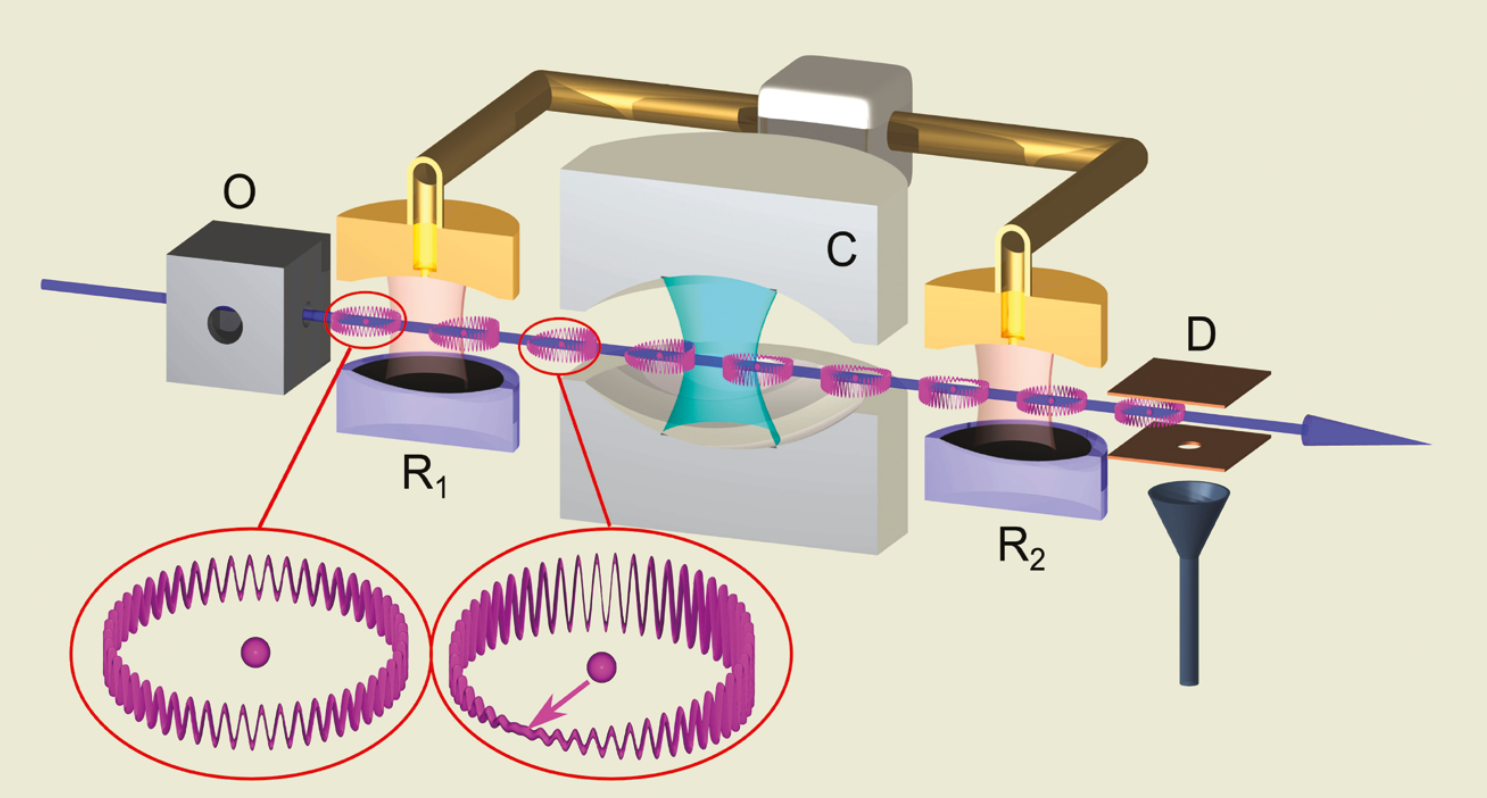
\includegraphics[width=0.5\textwidth]{images/aufbau.png}
		\caption{cQED Aufbau mit Ramsey Interferometer\cite{lect}}
	\end{figure}
\end{frame}
\section{Schrödingers Kätzchen}
\begin{frame}
	\frametitle{Schrödingers Kätzchen}
	\begin{itemize}
		\item Rydberg-Atom $\hat{=}$ Katze
		      \begin{itemize}
			      \item Zustand vom Rydberg-Atom gibt Aufschluss über Zustand von Photon
			      \item Zustand von Katze gibt Aufschluss über Zustand von Atom
		      \end{itemize}
	\end{itemize}
	\begin{columns}
		\begin{column}{0.45\textwidth}
			\begin{figure}
				\center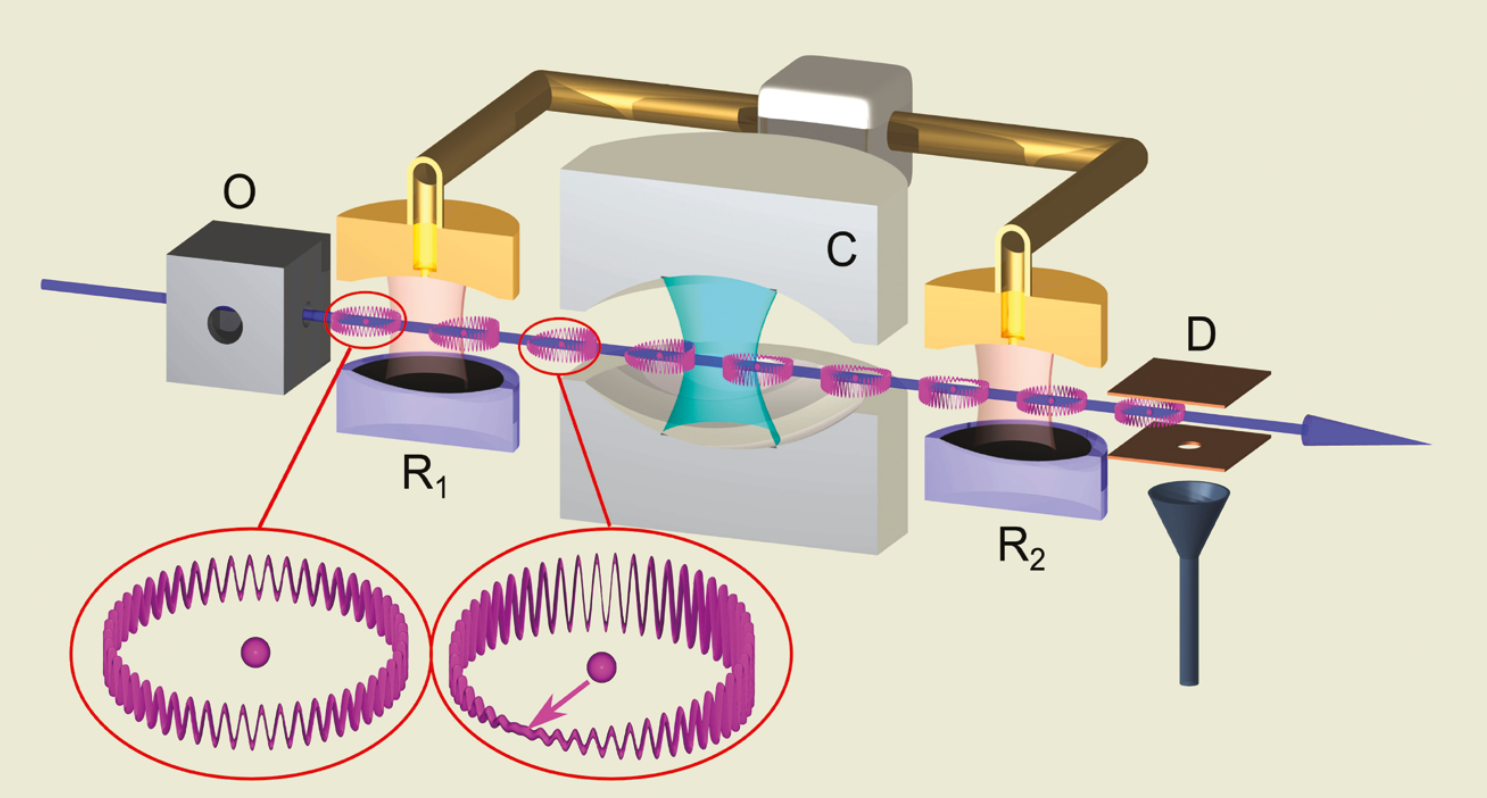
\includegraphics[width=1\textwidth]{images/aufbau.png}
				\caption{cQED Aufbau mit Ramsey Interferometer\cite{lect}}
			\end{figure}
		\end{column}
		\begin{column}{0.1\textwidth}
			\center$\Leftrightarrow$
		\end{column}
		\begin{column}{0.45\textwidth}
			\begin{figure}
				\center\includegraphics[width=0.8\textwidth]{scat.png}
				\caption{Schrödingers Katze\cite{lect}}
			\end{figure}
		\end{column}
	\end{columns}

\end{frame}
\section{Ergebnisse}
\begin{frame}{Ergebnisse}
    \begin{itemize}
      \item können so auf die Präsenz eines singulären Photons schließen
      \item kann aber auch so angepasst werden, dass verschiedene Dipolausrichtungen verschiedene Mengen an Photonen darstellen
    \end{itemize}
			\begin{figure}
				\center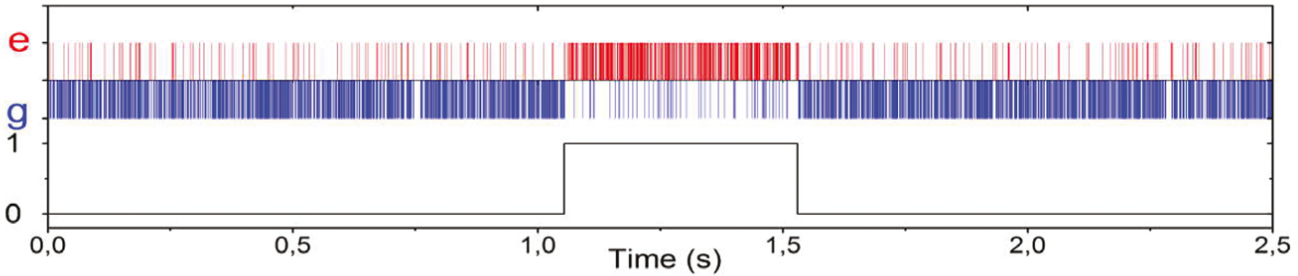
\includegraphics[width=1\textwidth]{detection.png}
				\caption{Aufnahme\cite{lect}}
			\end{figure}
\end{frame}
\begin{frame}{Ergebnisse}
			\begin{figure}
				\center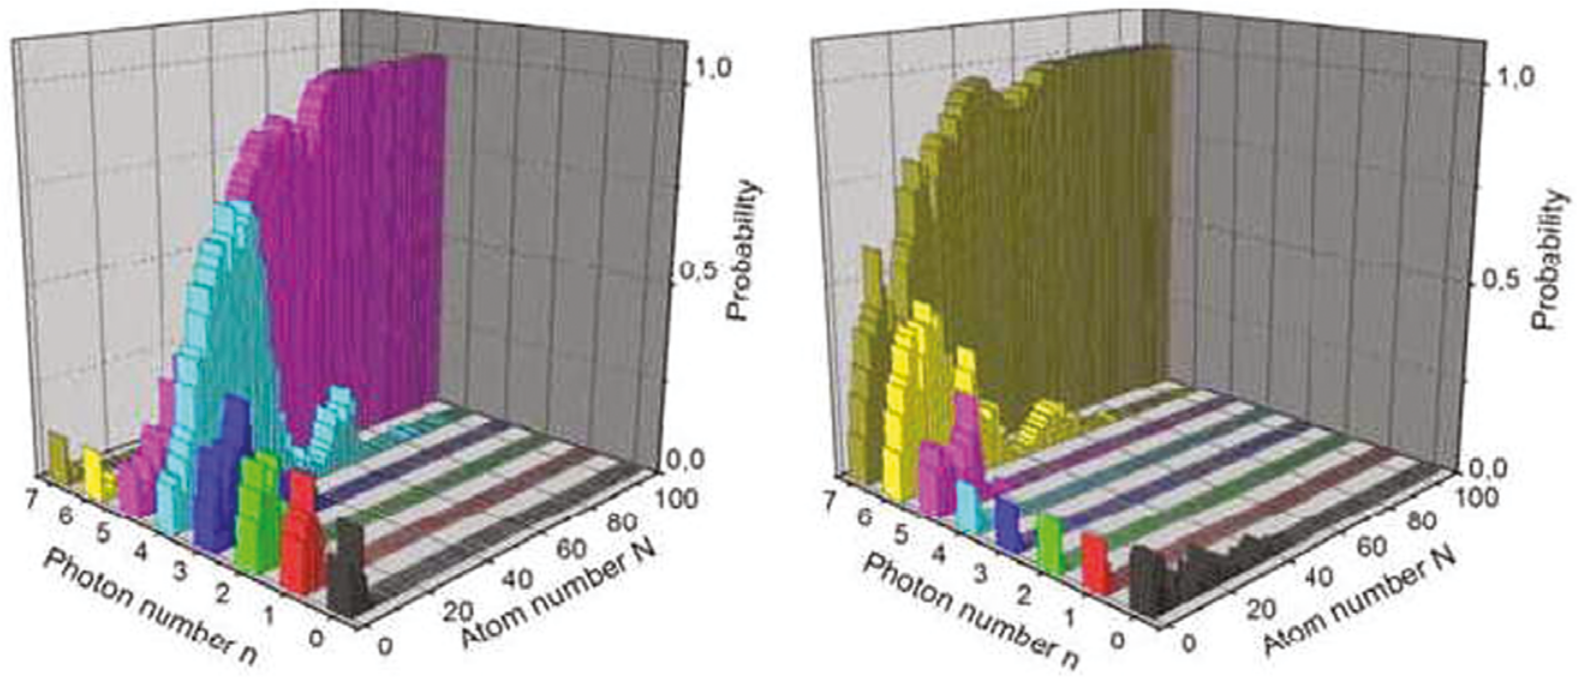
\includegraphics[width=1\textwidth]{multdet.png}
				\caption{Wahrscheinlichkeitsverteilung für die Photonenanzahl\cite{lect}}
			\end{figure}
\end{frame}
\begin{frame}{Ergebnisse}
			\begin{figure}
				\center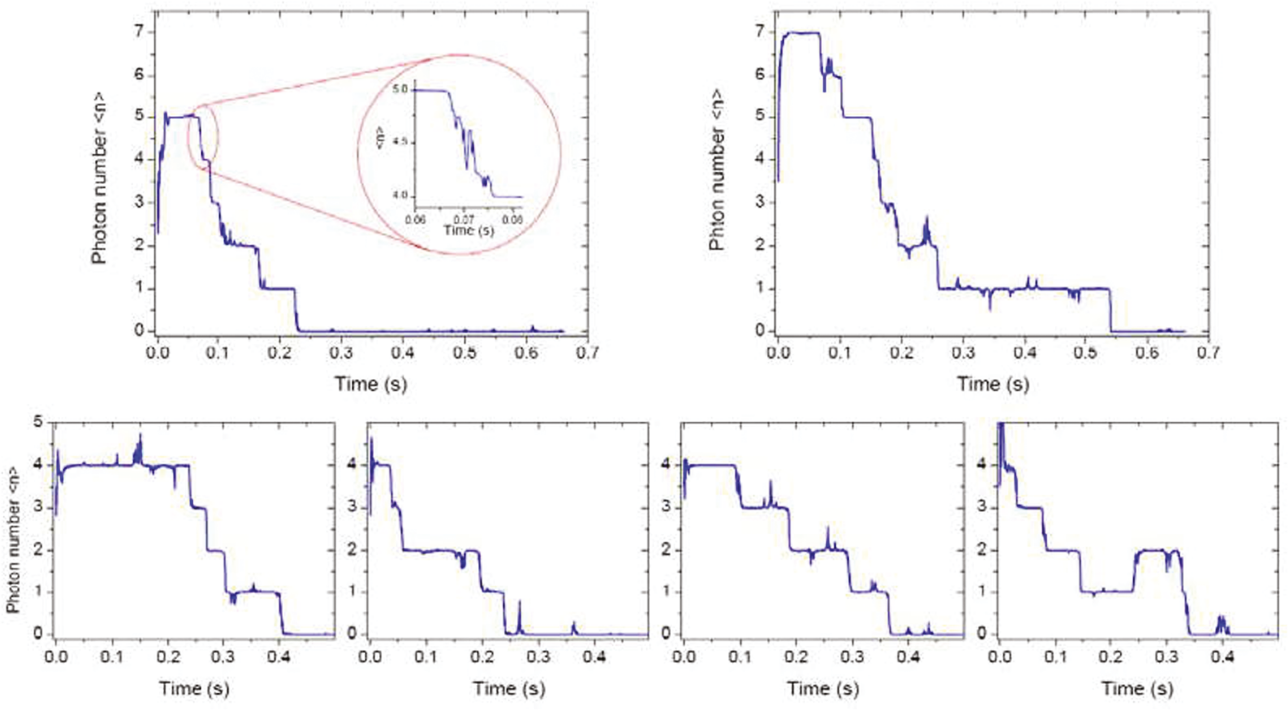
\includegraphics[width=1\textwidth]{timeevol.png}
				\caption{Zeitentwicklung\cite{lect}}
			\end{figure}
\end{frame}

\section{Zusammenfassung}
\begin{frame}{Zusammenfassung}
	\begin{itemize}
		\item Aparatur
		      \begin{itemize}
			      \item Cavity: Stehende Mikrowelle
			      \item QND: Rysberg-Atom in Superposition abhängig von Präsens von Photon
		      \end{itemize}
        \item Zum ersten Mal einzelnes Teilchen gemesse, ohne Zustand zu zerstören
        \item direkt analog zu bekanntem Gedankenexperiment: Schrödingers Katze
	\end{itemize}
\end{frame}
\begin{frame}
	\printbibliography
\end{frame}
\end{document}
